%------------------------------------------------------------------------------%
\documentclass[fleqn,utf8,aspectratio=169,12pt]{beamer}

\usepackage{calculo_varias_variaveis-1}

\title{Regra da Cadeia}

%------------------------------------------------------------------------------%
\begin{document}

\addtitle

%------------------------------------------------------------------------------%
\section{Regra da Cadeia}

%------------------------------------------------------------------------------%
\begin{frame}{Regra da Cadeia em uma variável}
  \[
    h(x) = f\big(g(x)\big)
  \]

  \pause
  \[
    h'(x)
    \;=\; f'\big(g(x)\big) \; g'(x)
  \]

  \pause
  \[
    \frac{dh}{dx}(x)
    \;=\; \frac{df}{dg}\big(g(x)\big) \; \frac{dg}{dx}(x)
  \]
\end{frame}

%------------------------------------------------------------------------------%
\section{Caso 1}

%------------------------------------------------------------------------------%
\begin{frame}{Regra da Cadeia -- Caso 1}
    Uma variável independente e duas variáveis intermediárias
    \vspace{\baselineskip}

    \pause
    Se \(w=f(x, y)\) é diferenciável
    \pause
    e se \(x=x(t)\) e \(y=y(t)\) são deriváveis

    \pause
    \vspace{.5\baselineskip}
    a composta \(w=f\big(x(t), y(t)\big)\) será uma função derivável de $t$ e
    \pause
    \[
        \frac{dw}{dt}(t)
        \;=\; \emph{\D{f}{x}\big(x(t), y(t)\big)}\; \frac{dx}{dt}(t)
        \;+\; \emph{\D{f}{y}\big(x(t), y(t)\big)}\; \frac{dy}{dt}(t)
    \]
\end{frame}

%------------------------------------------------------------------------------%
\begin{frame}{Regra da Cadeia -- Caso 1 -- 2D}
  \centering
  \large
  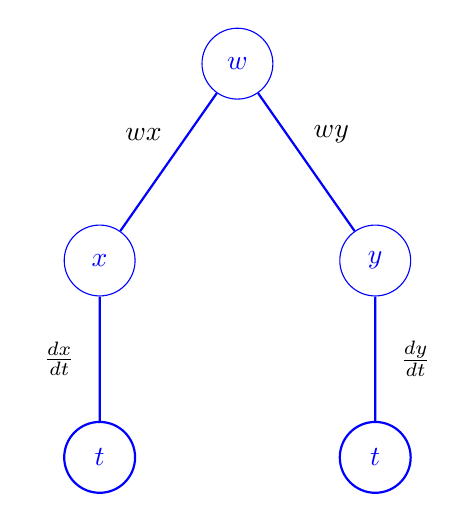
\begin{tikzpicture}[
    every node/.style={minimum size=9mm},
    level distance=25mm,
    level 1/.style={sibling distance=35mm},
    level 2/.style={sibling distance=25mm},
    edge from parent/.style={draw, blue, thick}
    ]

    \node[draw, circle, blue] {$w$}
    child {
      node[draw, circle, blue] {$x$}
      child {
        node[draw, circle, blue] {$t$}
        edge from parent node[left, midway, black] {$\frac{dx}{dt}\;$}
      }
      edge from parent node[left, pos=0.30, black] {$\D{w}{x}\;\;$}
    }
    child {
      node[draw, circle, blue] {$y$}
      child {
        node[draw, circle, blue] {$t$}
        edge from parent node[right, midway, black] {$\;\frac{dy}{dt}$}
      }
      edge from parent node[right, pos=0.30, black] {$\;\;\D{w}{y}$}
    };
  \end{tikzpicture}
\end{frame}

%------------------------------------------------------------------------------%
\include{ex/G-01-Regra-da-cadeia-ex1}

%------------------------------------------------------------------------------%
\begin{frame}{Com Três Variáveis}
    Se \(w=f(x, y, z)\) é diferenciável

    \pause
     e se \(x=x(t)\), \(y=y(t)\) e \(z=z(t)\) são deriváveis

    \pause
    a composta \(w=f\big(x(t), y(t), z(t)\big)\) será uma função derivável de $t$ e

    \pause
    \begin{align*}
        \frac{dw}{dt}(t)
        & = \emph{\D{f}{x}\big(x(t), y(t), z(t)\big)} \; \frac{dx}{dt}(t) \\[3mm]
        & + \emph{\D{f}{y}\big(x(t), y(t), z(t)\big)} \; \frac{dy}{dt}(t) \\[3mm]
        & + \emph{\D{f}{z}\big(x(t), y(t), z(t)\big)} \; \frac{dz}{dt}(t)
    \end{align*}
\end{frame}

%------------------------------------------------------------------------------%
\begin{frame}{Regra da Cadeia -- Caso 1 -- 3D}
  \centering
  \large
  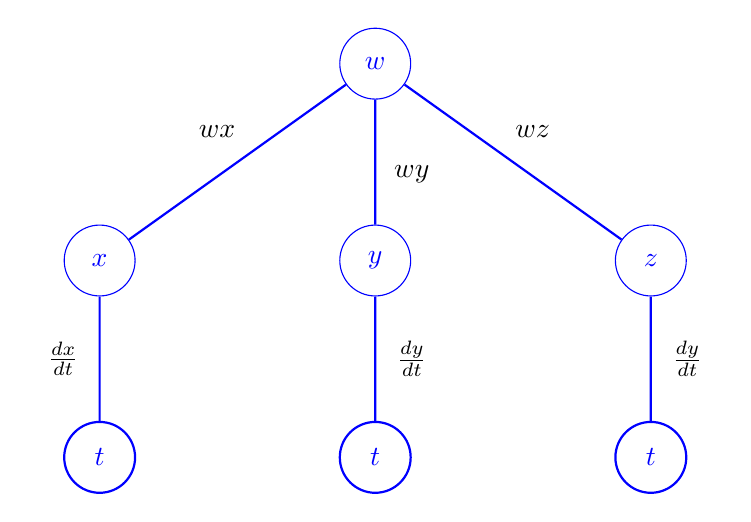
\begin{tikzpicture}[
    every node/.style={minimum size=9mm},
    level distance=25mm,
    level 1/.style={sibling distance=35mm},
    level 2/.style={sibling distance=25mm},
    edge from parent/.style={draw, blue, thick}
    ]

  \node[draw, circle, blue] {$w$}
  child {
    node[draw, circle, blue] {$x$}
    child {
      node[draw, circle, blue] {$t$}
      edge from parent node[left, midway, black] {$\frac{dx}{dt}$}
    }
    edge from parent node[left, pos=0.3, black] {$\D{w}{x}\quad$\;}
  }
  child {
    node[draw, circle, blue] {$y$}
    child {
      node[draw, circle, blue] {$t$}
      edge from parent node[right, midway, black] {$\frac{dy}{dt}$}
    }
    edge from parent node[right, pos=0.6, black] {$\D{w}{y}$}
  }
  child {
    node[draw, circle, blue] {$z$}
    child {
      node[draw, circle, blue] {$t$}
      edge from parent node[right, midway, black] {$\frac{dy}{dt}$}
    }
    edge from parent node[right, pos=0.3, black] {$\quad\;\D{w}{z}$}
  };


  \end{tikzpicture}
\end{frame}

%------------------------------------------------------------------------------%
\section{Caso 2}

%------------------------------------------------------------------------------%
\begin{frame}{Regra da Cadeia -- Caso 2}
    Funções definidas em superfícies
    \vspace{0.5\baselineskip}

    \pause
    Se \(w=f(x, y, z)\) é diferenciável

    \pause
    e se \(x=x(r, s)\), \(y=y(r, s)\) e \(z=z(r, s)\) são deriváveis

    \pause
    a composta \(w=f\big(x(r, s), y(r, s), z(r, s)\big)\)
    será uma função das deriváveis $r$ e $s$

    \pause
    e terá duas derivadas parciais
    \[
        \D{w}{r}
        = \emph{\D{f}{x}} \D{x}{r}
        + \emph{\D{f}{y}} \D{y}{r}
        + \emph{\D{f}{z}} \D{z}{r}
    \]
    \[
        \pause
        \D{w}{s}
        = \emph{\D{f}{x}} \D{x}{s}
        + \emph{\D{f}{y}} \D{y}{s}
        + \emph{\D{f}{z}} \D{z}{s}
    \]
\end{frame}

%------------------------------------------------------------------------------%

\begin{frame}{Regra da Cadeia -- Caso 2}
  \centering
  \large
  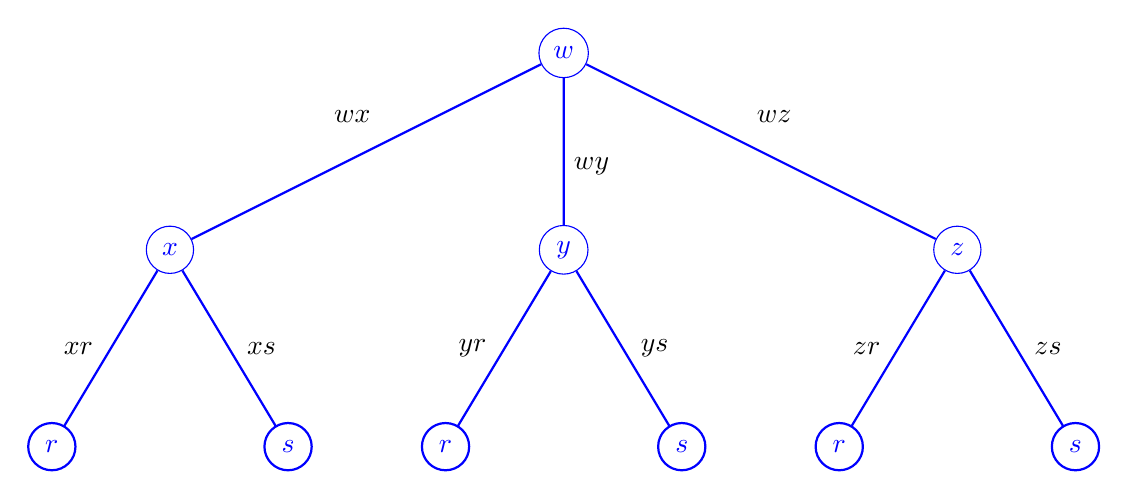
\begin{tikzpicture}[
    every node/.style={minimum size=6mm},
    level distance=25mm,
    level 1/.style={sibling distance=50mm},
    level 2/.style={sibling distance=30mm},
    edge from parent/.style={draw, blue, thick}
    ]

    \node[draw, circle, blue] {$w$}
    child {
      node[draw, circle, blue] {$x$}
      child {
        node[draw, circle, blue] {$r$}
        edge from parent node[left, midway, black] {$\D{x}{r}\;$}
      }
      child {
        node[draw, circle, blue] {$s$}
        edge from parent node[right, midway, black] {$\;\D{x}{s}$}
      }
      edge from parent node[left, pos=0.3, black] {$\D{w}{x}\qquad$}
    }
    child {
      node[draw, circle, blue] {$y$}
      child {
        node[draw, circle, blue] {$r$}
        edge from parent node[left, midway, black] {$\D{y}{r}\;$}
      }
      child {
        node[draw, circle, blue] {$s$}
        edge from parent node[right, midway, black] {$\;\D{y}{s}$}
      }
      edge from parent node[right, pos=0.6, black] {$\D{w}{y}$}
    }
    child {
      node[draw, circle, blue] {$z$}
      child {
        node[draw, circle, blue] {$r$}
        edge from parent node[left, midway, black] {$\D{z}{r}\;$}
      }
      child {
        node[draw, circle, blue] {$s$}
        edge from parent node[right, midway, black] {$\;\D{z}{s}$}
      }
      edge from parent node[right, pos=0.3, black] {$\qquad\D{w}{z}$}
    };

  \end{tikzpicture}
\end{frame}

%------------------------------------------------------------------------------%
\section{Exemplos}

\include{ex/G-01-Regra-da-cadeia-ex2}
\include{ex/G-01-Regra-da-cadeia-ex3}
\include{ex/G-01-Regra-da-cadeia-ex4}
\include{ex/G-01-Regra-da-cadeia-ex5}
\include{ex/G-01-Regra-da-cadeia-ex6}

%------------------------------------------------------------------------------%
\section{Lista Mínima}

%------------------------------------------------------------------------------%
\begin{frame}{Lista Mínima}
  Cálculo Vol. 2 do Thomas 12\textsuperscript{a} ed. -- Seção 14.4
  \begin{enumerate}
    \item Estudar o texto da seção
    \item Resolver os exercícios: 3, 5, 6, 10, 12, 14, 17
  \end{enumerate}

  \vfill
  Atenção: A prova é baseada no livro, não nas apresentações
\end{frame}

%------------------------------------------------------------------------------%
\end{document}
%------------------------------------------------------------------------------%
